% LaTeX Template f�r Datenstrukturen und Algorithmen Abgaben
% Autor: Sandro Speth
% Bei Fragen: Sandro.Speth@studi.informatik.uni-stuttgart.de
\documentclass[12pt]{article}
\usepackage[latin1]{inputenc}
\usepackage[T1]{fontenc}
\usepackage[ngerman]{babel}
\usepackage{graphicx}
\usepackage{color}
\usepackage{listings}
\usepackage[a4paper,lmargin={2cm},rmargin={2cm},tmargin={3.5cm},bmargin = {2.5cm},headheight = {4cm}]{geometry}
\usepackage{amsmath,amssymb,amstext}
\usepackage{amsthm}
\usepackage[lined,algonl,boxed]{algorithm2e}
\usepackage{tikz}
\usepackage[inline]{enumitem}
\usepackage{tikz}
\usetikzlibrary{trees}
\usepackage{fancyhdr}
\usepackage{forest}
\pagestyle{fancy} 
\fancyhf{}

\renewcommand{\theenumi}{(\alph{enumi})}
\renewcommand{\labelenumi}{\text{\theenumi}}

\newcounter{sheetnr}
\setcounter{sheetnr}{06} % Nummer des �bungsblattes

\newcounter{exnum}
\setcounter{exnum}{1} % Nummer der Aufgabe

\newcommand{\aufgabe}[1]{\section*{Aufgabe \theexnum\stepcounter{exnum}: #1}} % Befehl f�r Aufgabentitel

% Rechter Teil der Kopfzeile:
% Namen und Matrikelnummern aller Bearbeiter
\rhead{Wilhelm Buchm�ller (3133783)\\
Artur Frenzen (2736424)\\
Daniel Wanner (3149308)}
 
% Linker Teil der Kopfzeile
\lhead{Datenstrukturen \& Algorithmen\\
Sommersemester 2016\\
�bungsblatt \thesheetnr}

% Beginn des eigentlichen Dokuments
\begin{document}
% Aufgabe 2
\aufgabe{Graphenrepr�sentation}
\begin{enumerate}
	\item 
	
	\begin{itemize}

	\item \(G_1\) ist gerichtet
	
	\item \(G_1\) ist gewichtet
	
	\item \(G_2\) ist gerichtet
	
	\item \(G_2\) ist nicht gewichtet
	
\end{itemize}

	\item
	
	\begin{tikzpicture}
		\begin{scope}[every node/.style={circle,thick,draw}]
    \node (D) at (0,0) {D};
    \node (A) at (0,3) {A};
    \node (F) at (2.5,0) {F};
    \node (B) at (5,0) {B};
    \node (E) at (8,0) {E};
    \node (C) at (8,3) {C} ;
	\end{scope}

	\begin{scope}[>={stealth[black]},
              every node/.style={fill=white,circle},
              every edge/.style={draw=red,very thick}]
    \path [->] (D) edge node {$8$} (A);
	\path [->] (C) edge node {$4$} (A);	
    \path [->] (C) edge [bend right = 20] node {$6$} (E);
    \path [->] (E) edge [bend right = 20] node {$1$} (C);
    \path [->] (B) edge node {$7$} (F);
    \path [->] (E) edge node {$6$} (B);
    
    
    
\end{scope}
\end{tikzpicture}

\hspace{10mm}


\begin{tikzpicture}
		\begin{scope}[every node/.style={circle,thick,draw}]
    \node (1) at (0,15) {1};
    \node (2) at (5,15) {2};
    \node (3) at (10,15) {3};
    \node (4) at (15,15) {4};
    \node (5) at (0,10) {5};
    \node (6) at (5,10) {6} ;
    \node (7) at (10,10) {7} ;
    \node (8) at (15,10) {8} ;
    \node (9) at (0,5) {9} ;
    \node (10) at (5,5) {10} ;
    \node (11) at (10, 5) {11} ;
    \node (12) at (15,5) {12} ;
    \node (13) at (13,3) {13} ;
	\end{scope}

	\begin{scope}[>={stealth[black]},
              every node/.style={fill=white,circle},
              every edge/.style={draw=red,very thick}]
    \path [->] (1) edge (2);
    \path [->] (1) edge [bend right=20] (3);
    \path [->] (1) edge [bend right=30] (4);
		\path [->] (2) edge (6);
		\path [->] (2) edge (11);
		\path [->] (4) edge (8);
		\path [->] (5) edge (6);
		\path [->] (5) edge (10);
		\path [->] (10) edge (7);
		\path [->] (7) edge (12);    
		\path [->] (8) edge (9);
		\path [->] (9) edge (13);
		\path [->] (12) edge [bend left=20] (9);
		
    
\end{scope}
\end{tikzpicture}
\item
\begin{tikzpicture}
	
\begin{scope}
	\node[draw] (A) at (0,0) {A};
	\node[draw] (B) at (0,-1) {B};
	\node[draw] (C) at (0,-2) {C};
	\node[draw] (D) at (0,-3) {D};
	\node[draw] (E) at (0,-4) {E};
	\node[draw] (F) at (0,-5) {F};
	
	\node[draw] (BF) at (1,-1) {F};
	\node[draw] (CA) at (1,-2) {A};
	\node[draw] (CE) at (2,-2) {E};
	\node[draw] (DA) at (1,-3) {A};
	\node[draw] (EB) at (1,-4) {B};
	\node[draw] (EC) at (2,-4) {C};
	\node[draw] (EC) at (2,-4) {C};
	
	
\end{scope}

\begin{scope}[>={stealth[black]}, every edge/.style={draw=black,very thick}]

    \path [->] (B) edge (BF);
		\path [->] (C) edge (CA);
		\path [->] (CA) edge (CE);
		
    \path [->] (D) edge (DA);
    \path [->] (E) edge (EB);
    \path [->] (EB) edge (EC); 
			
    \path [->] (A) edge (B);    
    \path [->] (B) edge (C);    
    \path [->] (C) edge (D);    
    \path [->] (D) edge (E);    
    \path [->] (E) edge (F);    
    
    
\end{scope}

\end{tikzpicture}

\item 
\(G_2\) = (13,19 | \underline{3,2,3,4} , \underline{2,3,6}, \underline{0} \underline{1,8}, \underline{2,6,10} \underline{0}, \underline{1, 12}, \underline{0}, \underline{1,13},\underline{0}, \underline{1,8}, \underline{2,11,9} \underline{0})

\end{enumerate}



% Aufgabe 2
\aufgabe{Breitensuche}
% Teilaufgaben
\begin{enumerate}
	\item F \(\rightarrow\) A \(\rightarrow\) E \(\rightarrow\) B \(\rightarrow\) X \(\rightarrow\) C \(\rightarrow\) D
	\item D \(\rightarrow\) C \(\rightarrow\) E \(\rightarrow\) X \(\rightarrow\) F \(\rightarrow\) A \(\rightarrow\) B
\end{enumerate}

\centering


\newpage


%\newpage
% Aufgabe 3
\aufgabe{Pr�fix/Patricia-Baum}
\begin{figure}[!h]
\centering


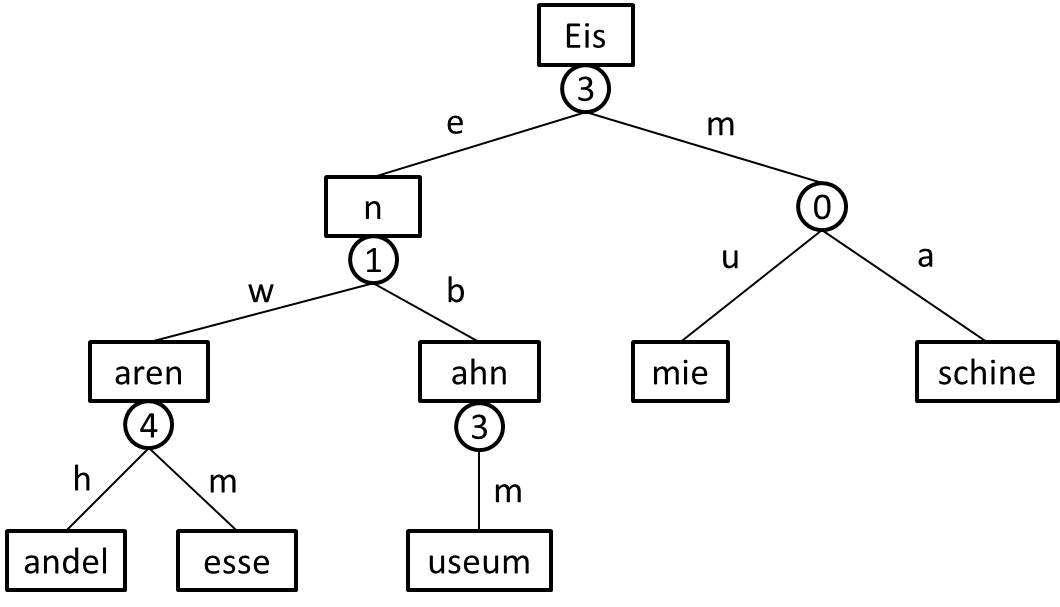
\includegraphics[width=\linewidth]{aufg3a_prefixbaum.jpg}

\caption{Teilaufgabe a)}
\label{fig:baum}
\end{figure}
\begin{figure}[!h]
\centering


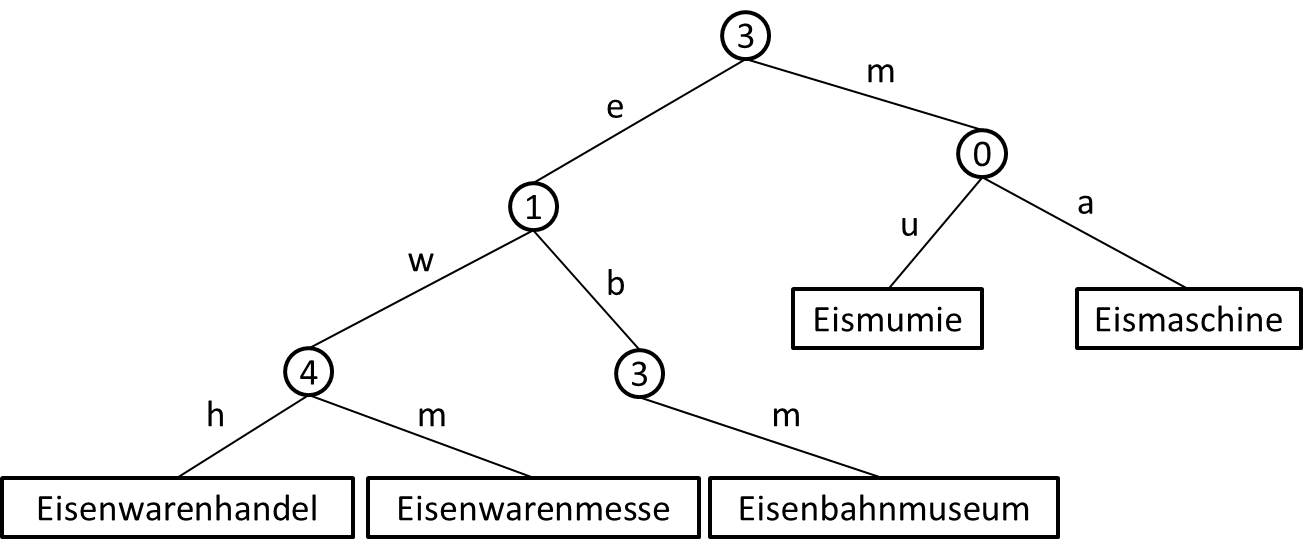
\includegraphics[width=\linewidth]{aufg3b_patriciabaum.jpg}


\caption{Teilaufgabe b)}
\label{fig:baum}
\end{figure}



% Ende des Dokuments
\end{document}
